\documentclass[portuguese,11pt,a4paper,titlepage]{article}

\usepackage{graphicx}
\usepackage{fancyhdr}
\usepackage[portuguese]{babel}
\usepackage{blindtext}
\usepackage{listings}
\usepackage[T1]{fontenc}
\usepackage[margin=2.5cm]{geometry}
\usepackage[final]{pdfpages}
\usepackage{siunitx}
\usepackage[framed, numbered]{matlab-prettifier}
\usepackage{wrapfig}
\usepackage{subcaption}
\usepackage{hyperref}

\hypersetup{
    colorlinks,
    citecolor=black,
    filecolor=black,
    linkcolor=black,
    urlcolor=black
}

\setlength{\headheight}{14.2pt}
\fancypagestyle{fancy}{
	\fancyhf{}
	\fancyhead[C]{A02 -- word\_ladder}
	\fancyfoot[R]{
		\textsf{\thepage}
	}
	\fancyfoot[L]{
		\textsf{AED -- 2022/2023}
	}
	\fancyfoot[C]{
\includegraphics[height=.6cm]{assets/ua.pdf}}
	\renewcommand{\headrulewidth}{0pt}
}
\pagestyle{fancy}

\definecolor{mygreen}{rgb}{0,0.6,0}
\definecolor{mygray}{rgb}{0.5,0.5,0.5}
\definecolor{mymauve}{rgb}{0.58,0,0.82}

\lstdefinestyle{c_without_comments}
{
	style=c_with_comments,
	morecomment  = [l][\@gobble]{//},
	morecomment  = [is]{/*}{*/},
}

\lstset{ 
	backgroundcolor=\color{white},   % choose the background color; you must add \usepackage{color} or \usepackage{xcolor}; should come as last argument
	basicstyle=\small\ttfamily,      % the size of the fonts that are used for the code
	breakatwhitespace=false,         % sets if automatic breaks should only happen at whitespace
	breaklines=true,                 % sets automatic line breaking
	captionpos=b,                    % sets the caption-position to bottom
	commentstyle=\color{mygreen},    % comment style
	extendedchars=true,              % lets you use non-ASCII characters; for 8-bits encodings only, does not work with UTF-8
	frameround=tttt,
	frame=single,	                 % adds a frame around the code
	keepspaces=true,                 % keeps spaces in text, useful for keeping indentation of code (possibly needs columns=flexible)
	keywordstyle=\color{blue},       % keyword style
	language=C,                      % the language of the code
	morekeywords={*,\ldots},         % if you want to add more keywords to the set
	numbers=none,                    % where to put the line-numbers; possible values are (none, left, right)
	rulecolor=\color{black},         % if not set, the frame-color may be changed on line-breaks within not-black text (e.g. comments (green here))
	showspaces=false,                % show spaces everywhere adding particular underscores; it overrides 'showstringspaces'
	showstringspaces=false,          % underline spaces within strings only
	showtabs=false,                  % show tabs within strings adding particular underscores
	stringstyle=\color{mymauve},     % string literal style
	tabsize=2,                       % sets default tabsize to 2 spaces
	literate=
		{Á}{{\'A}}1
		{Â}{{\^A}}1
		{á}{{\'a}}1
		{à}{{\`a}}1
		{ã}{{\~a}}1
		{â}{{\^a}}1
		{É}{{\'E}}1
		{Ê}{{\^E}}1
		{è}{{\`e}}1
		{é}{{\'e}}1
		{ê}{{\^e}}1
		{Í}{{\'I}}1
		{Ì}{{\`I}}1
		{í}{{\'i}}1
		{î}{{\^i}}1
		{Ó}{{\'O}}1
		{Õ}{{\~O}}1
		{Ô}{{\^O}}1
		{ò}{{\`o}}1
		{ó}{{\'o}}1
		{õ}{{\~o}}1
		{ô}{{\^o}}1
		{Ú}{{\'U}}1
		{Ù}{{\`U}}1
		{ù}{{\`u}}1
		{ú}{{\'u}}1
		{ü}{{\"u}}1
		{ç}{{\c{c}}}1
}

\newcommand{\foreign}[1]{\textit{#1}}
\newcommand{\srcdir}{..}
\newcommand{\hashtablegrowdir}{\srcdir/hash\_table\_grow-test}
\setcounter{secnumdepth}{2}

\title{ \normalsize Licenciatura em Engenharia Informática\vskip 1.5em
		\Huge Algoritmos e Estruturas de Dados\vskip .7em
		\bfseries Word Ladder\vskip 1.5em
		
\includegraphics{assets/ua.pdf}
}
\author{
	João Catarino\\NMec: 93096\and Rúben Garrido\\NMec: 107927\and Nuno Vieira\\NMec: 107283
}
\date{\today}
\addto\captionsportuguese{\renewcommand*\contentsname{Índice}}

\begin{document}
\maketitle

\tableofcontents
\pagebreak

\section{Introdução}
Este trabalho centra-se no estudo de dicionários de palavras, interpretando cada um como um grafo não-orientado, onde cada nó representa uma palavra. Palavras que diferem num só caracter são unidas por um arco.
Deste modo, é possível determinar \textit{word ladders} entre palavras: os caminhos mais curtos entre elas, compostos por outras palavras. Por exemplo, \textit{tudo, todo, nodo, nado, nada} é uma \textit{word ladder} entre as palavras \textit{tudo} e \textit{nada}.
Os objetivos deste trabalho incluem implementar uma \textit{hash table}, a representação de um grafo não-orientado e a estrutura de dados \textit{union find}, bem como determinar o componente complexo de uma palavra, o diâmetro de um componente conexo e a maior \textit{word ladder} existente no dicionário fornecido.

\section{Representação do problema}
A implementação do grafo foi feita através de uma \textit{linked hash table}, uma vez que esta possui uma complexidade computacional \begin{math}O(1)\end{math} para a inserção e procura de elementos.
Esta complexidade computacional é importante, dado que a geração de arcos entre palavras implica verificar se todas a permutações de mudança de um caracter de um nó correspondem a palavras contidas no dicionário. Para além disso, caso a complexidade computacional fosse \begin{math}O(n)\end{math} e existisse um número avultado de palavras, a \textit{word ladder} poderia demorar algum tempo a ser gerada.

A \textit{linked hash table} é composta por um array de \textit{buckets}: \textit{linked lists} que contêm nós.
Nós aos quais sejam atribuidos o mesmo índice de array pela função de dispersão são colocados no inicio da lista presente nesse índice.
Cada nó contém uma \textit{linked list} onde são guardadas referências aos nós adjacentes. A figura \ref{fig:hash_table} mostra a estrutura da \textit{hash table}.

\begin{figure}[h]
	\centering
	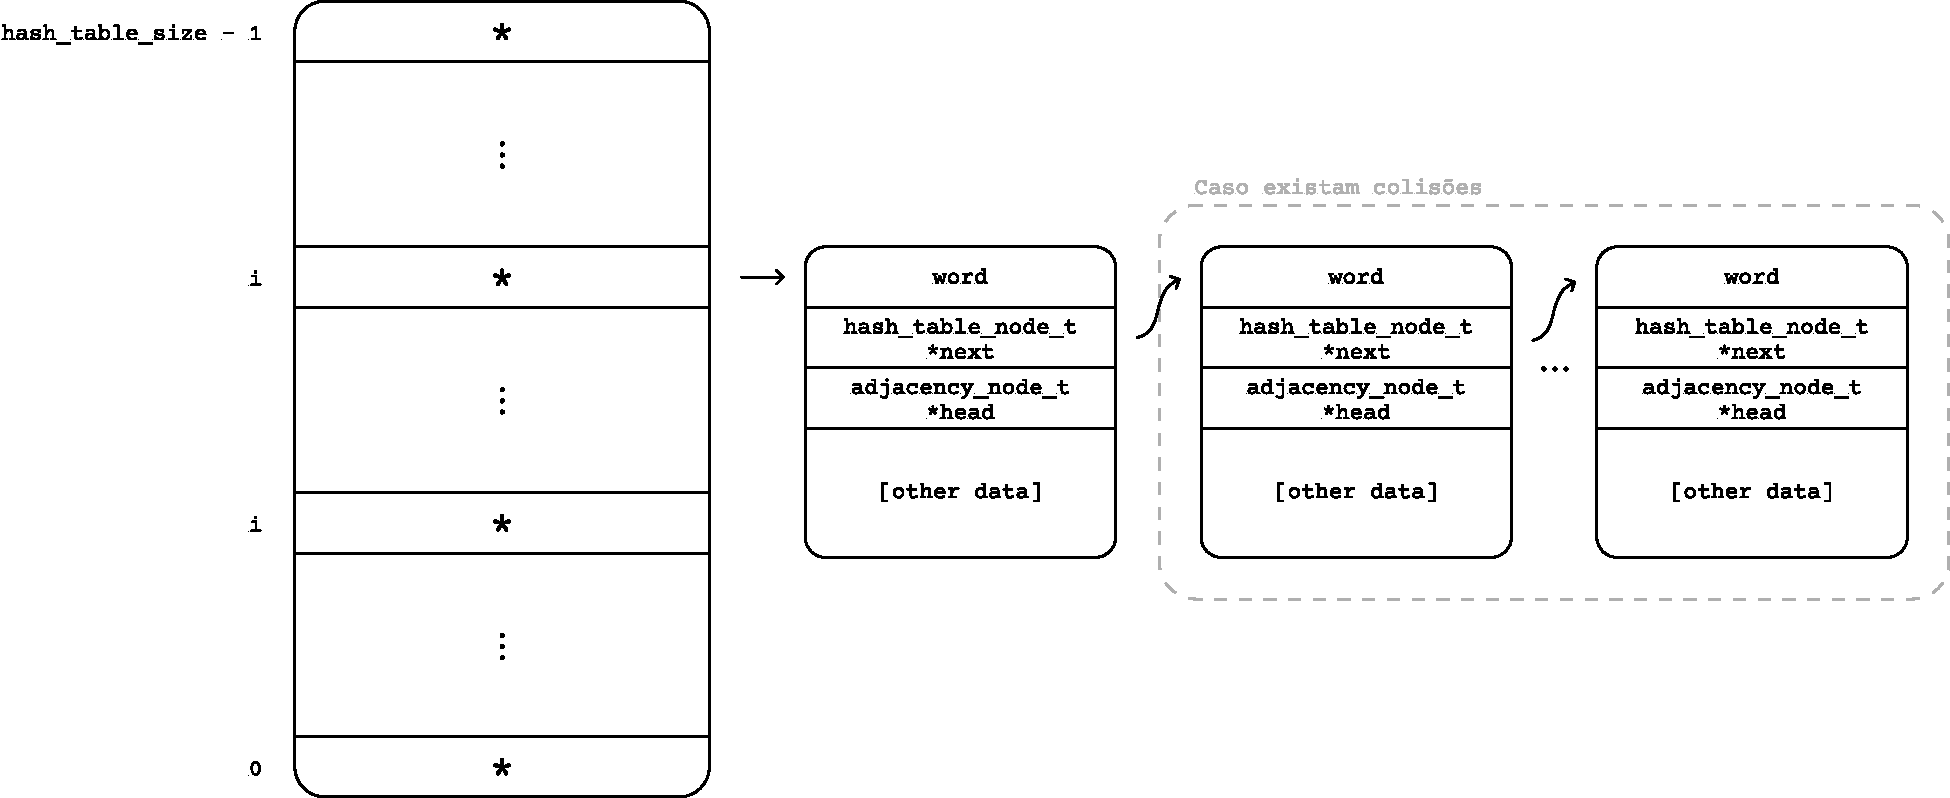
\includegraphics[width=\textwidth]{assets/hash_table-structure.pdf}
	\caption{Estrutura da \textit{hash table}}
	\label{fig:hash_table}
\end{figure}

Os índices são calculados através do resto da divisão entre o valor retornado por uma \textit{hash function} e o tamanho da \textit{hash table}. A \textit{hash function} utilizada faz uso do algoritmo \verb|CRC32| (acrónimo de \textit{Cyclic Redudancy Check}, 32 bits).

\section{Implementação}
\subsection{Funções de \textit{hash table}}

\subsubsection{hash\_table\_create}
Esta função aloca memória para uma estrutura de dados do tipo definido \verb|hash_table_t|, que representa a \foreign{hash table}, e para o seu \foreign{array} interno \verb|heads| que irá conter as entradas da tabela. O tamanho inicial da tabela é definido no macro
\verb|_hash_table_init_size_| e as suas entradas são inicializadas a zero de forma implícita pela
função \verb|calloc|. No final, é guardado o tamanho inicial da tabela na estrutura de dados. A função termina o programa se uma das alocações não for bem sucedida.

\subsubsection{hash\_table\_grow}
\verb|hash_table_grow| é a função responsável por aumentar o tamanho da \foreign{hash table}. A sua condição de incremento depende do rácio entre o tamanho desta e o número de colisões, onde, caso seja superior a 5, verificar-se-á o incremento. A função inicializa uma nova tabela (com um tamanho igual ao dobro da anterior) usando a função \verb|calloc| e, para cada \textit{node} desta, recalcula o seu índice, através da função \verb|crc32|, e insere-o na nova tabela. Por fim, os endereços para o array \verb|heads| e para o tamanho da tabela (\verb|hash_table_size|) são atualizados.

\subsubsection{hash\_table\_free}
Esta função desaloca a memória previamente reservada para a \foreign{hash table} e outras
estruturas de dados nela contidas. Esta começa por iterar sobre todas as posições do \foreign{array}, chamando a função \verb|free_hash_llist|, libertando a \foreign{linked list} nessa posição. Por sua vez, esta irá iterar sobre todos os nós da lista através
do ponteiro \verb|next| e chamar a função \verb|free_hash_table_node| sobre cada nó, que irá primeiro libertar a lista de adjacência com a função \verb|free_adjacency_llist| e depois o próprio nó. A função \verb|free_adjacency_llist| simplesmente itera sobre todos
os membros da lista ligada e liberta cada um deles.

\subsubsection{create\_word\_node}
Cria um novo nó de \textit{hash table} com a palavra fornecida como argumento. Este nó, cuja memória alocada é obtida através da função \verb|allocate_hash_table_node|, é inicializado com a palavra e alguns parâmetros predefinidos. Por fim, a função retorna o endereço do \textit{node} recém-criado.

\subsection{Funções de grafo}

\subsubsection{find\_word}
Função dedicada à procura e inserção de elementos na \foreign{hash table}. 
É calculado o índice, que resulta do resto da divisão entre o resultado da aplicação da \foreign{hash function} à palavra desejada e o tamanho máximo da tabela. Esta operação distribui o indice da palavra entre 0 e o tamaho da tabela. De seguida, a função itera sobre a lista ligada na posição calculada, procurando um nó igual através da função \verb|strcmp|, e retorna-o se for o caso.
Caso a palavra não exista e a opção \verb|insert_if_not_found| seja verdadeira, o programa aloca um novo nó para a palavra através da função \verb|create_word_node| e coloca-o na lista ligada, atualizando os valores estatísticos na \foreign{hash table}.

\subsubsection{similar\_words}
É responsável por encontrar palavras semelhantes à palavra fornecida como argumento. A verificação é baseada em caracteres \textit{Unicode}, onde, para cada caracter da palavra, este é substituído pelos vários caracteres aceites. Caso a nova palavra exista na \foreign{hash table}, é efetuada uma chamada à função \verb|add_edge| (ver secção \ref{sssec:addedge}). A função termina quando não existirem mais caracteres para substituir.

\subsubsection{find\_representative}
Função responsável pela determinação do nó representante do componente conexo de um nó requisitado. Antes de devolver o resultado, a função atualiza os representates dos nós percorridos anteriormente.

O seu funcionamento consiste em iterar sobre o representante do nó dado como argumento recursivamente até que o representante de um nó seja ele próprio.
Após determinar o representante, esta parte novamente do nó passado como argumento e altera o representante de forma recursiva para o anteriormente determinado até chegar a este novamente.
Desta forma, o caminho para o representante é simplificado e as chamadas posteriores com o mesmo nó como argumento serão mais rápidas.

\subsubsection{add\_edge}\label{sssec:addedge}
Esta função tenta adicionar um arco entre um nó existente e uma palavra que pode não existir, para além de implementar os aspetos da estrutura de dados \textit{Union-Find}.
Esta começa por procurar a \textit{string} dada no grafo, retornando caso não a encontre. Caso contrário, procura o segundo nó na lista de adjacência do primeiro e retorna se for o caso, para garantir que o arco não é duplicado.
Ao adicionar o arco, é incrementado o contador de arcos da tabela e são adicionados nós de adjacência às tabelas de adjacência das palavras.

A função \verb|insert_edge| trata de alocar o nó de adjacência para cada vértice e de os colocar nas listas respetivas. Neste sentido, a função trata de executar a operação \foreign{Union} entre os conjuntos (componentes conexos) de cada vértice.
Primeiro, são determinados os representantes de cada um através da função
\verb|find_representative| vista anteriormente. Se estes forem diferentes, a operação ocorre. Para minimizar o tamanho do caminho de representantes, o nó com menos vértices na altura da operação é escolhido como o representante do novo componente conexo. Finalmente, são somados os numeros de vértices e arcos, é decrementado o número de componentes e é atualizado o tamanho do maior componente.

\subsubsection{breadh\_first\_search}
A função \verb|breadh_first_search|, cujos argumentos são o número máximo de vértices, uma lista de vértices, o array de origem e o ponto de destino, tem como objetivo retornar o número de vértices visitados. Se for especificado o destino, será possível obter o 
caminho mais curto até este seguindo recursivamente o seu ponteiro \verb|previous|. Para
este efeito, é utilizado o algoritmo \textit{Breadth-first search}. Este percorre uma
árvore nivel a nivel, garantindo o menor percurso para cada nó visitado. Foi implementada para este caso
uma \foreign{queue} circular, de forma a garantir que o tamanho máximo desta é constante.

Em primeiro lugar, é efetuada uma chamada à função \verb|allocate_ptr_queue| -- que devolve uma \textit{queue} --, e uma chamada à função \verb|queue_put_hi|, que aceita como parâmetros de entrada a \textit{queue} e o array de origem. De seguida, dentro de um ciclo \verb|while| onde o tamanho da \textit{queue} é positivo, é incrementado os valores de \verb|visited| e \verb|list_len|, e, num ciclo \verb|for|, são atualizados os valores e endereços de \verb|vertex->visited| e \verb|vertex->previous|.

\subsection{Funções de \textit{queue}}
\subsubsection{allocate\_ptr\_queue}
Esta função aloca memória para uma \textit{queue} de ponteiros. Esta operação começa
por alocar memória para a estrutura de metadados da \foreign{queue}, que contêm as
variáveis necessárias para o manipulamento de uma \foreign{queue}. Posteriormente,
é alocado o \foreign{array} circular de ponteiros. Finalmente, são inicializadas
as variáveis de controlo da estrutura de dados e o seu ponteiro é devolvido.

\subsubsection{free\_ptr\_queue}
A função que liberta a memória alocada para a \foreign{queue}. Isto implica apenas
libertar o seu \foreign{array} circular e finalmente a própria estrutura.

\subsubsection{queue\_put\_hi}
Implementação da operação \foreign{enqueue}, onde um elemento, neste
caso um ponteiro, é adicionado ao final da fila. A função começa por executar um
\foreign{assert} para assegurar que o tamanho da fila não é ultrapassado. Depois,
é inserido o novo elemento na posição \foreign{hi}. Este valor não representa na
verdade o final da fila, mas sim a posição imediatamente asseguir. O valor é agora
incrementado e assume o valor do resto da sua divisão pelo tamanho máximo da 
\foreign{queue}. Isto implica que para valores menores que o maior índice possível, \foreign{hi} mantem-se, caso contrário, volta à posição 0, garantindo a circularidade.

\subsubsection{queue\_get\_lo}
Implementação da operação \foreign{dequeue}, onde o elemento inicial da fila é
removido e devolvido. A operação começa por um \foreign{assert}, para garantir
que o programa não tenta remover um elemento de uma fila vazia. De seguida, o valor
na posição \foreign{lo} é guardado numa variável temporária. Isto é feito porque
o inicio da fila pode ``saltar'' para o outro lado após a sua incrementação. Tendo
o valor guardado, é atualizada a posição \foreign{lo} da mesma forma como na função
\verb|queue\_put\_hi|. No final, é devolvido o valor guardado.

\section{\textit{Word ladders} interessantes}
\subsection{Palavras com 4 letras}
A maior \textit{word ladder} encontrada ocorre entre as palavras ``Kong'' e ``está'':
\begin{enumerate}
	\itemsep 0em
	\item Kong
	\item King
	\item Ping
	\item Pina
	\item tina
	\item tino
	\item tipo
	\item aipo
	\item arpo
	\item arpe
	\item arte
	\item ante
	\item ente
	\item este
	\item está
\end{enumerate}

\section{Verificação de \textit{memory leaks}}
Para verificar se existem \textit{memory leaks} no programa criado, foi utilizado o \foreign{Valgrind}, um programa constituído por um conjunto de ferramentas para a deteção de erros de memória e de \foreign{threading}. Para o efeito, foi utilizado o \foreign{Memcheck}, que é uma ferramenta para deteção de erros de memória.

Obteve-se o seguinte resultado, para o programa \verb|solution_word_ladder.c|, com o ficheiro \verb|wordlist-four-letters.txt| como argumento:

\begin{verbatim}
==500745== Memcheck, a memory error detector
==500745== Copyright (C) 2002-2022, and GNU GPL'd, by Julian Seward et al.
==500745== Using Valgrind-3.19.0 and LibVEX; rerun with -h for copyright info
==500745== Command: ./solution_word_ladder wordlist-four-letters.txt
==500745== 
Your wish is my command:
  1 WORD       (list the connected component WORD belongs to)
  2 FROM TO    (list the shortest path from FROM to TO)
  3 WORD       (list component info)
  4            (list hash table info)
  5            (list graph info)
  0            (terminate)
> 0
==500745== 
==500745== HEAP SUMMARY:
==500745==   in use at exit: 0 bytes in 0 blocks
==500745==   total heap usage: 27,700 allocs, 27,700 frees, 60,322,800 bytes
             allocated
==500745== 
==500745== All heap blocks were freed -- no leaks are possible
==500745== 
==500745== ERROR SUMMARY: 0 errors from 0 contexts (suppressed: 0 from 0)
\end{verbatim}

Assim, concluímos que não existem \textit{memory leaks} no programa. 

\pagebreak
\section{Análise do incremento da \textit{hash table}}
Por padrão, o tamanho inicial da \textit{hash table} é 1000. No entanto, quando o número de entradas começa a ser significativo, começam a surgir colisões, o que implica uma perca da complexidade computacional \begin{math}O(1)\end{math}. Para evitar este problema, quando o rácio entre o tamanho da \textit{hash table} e o número de colisões é superior a 5, o tamanho da \textit{hash table} é incrementado, através da função \verb|hash_table_grow|, que recebe como argumento a referida \textit{hash table}.

Contudo, a escolha do fator de incremento deve ser ponderada, já que, se for muito pequeno, o número de colisões diminui pouco, e se for muito grande, existe demasiada memória alocada não utilizada, o que leva a um desperdício de recursos. É esta escolha que pretendemos analisar.

\subsection{Explicação do código}
Foi desenvolvida uma nova função \verb|hash_table_grow|, num programa à parte, em que, após ser verificada a condição de incremento (rácio entre o tamanho da \textit{hash table} e o número de colisões), é percorrido um ciclo \verb|for|, onde são testados vários valores de \verb|j| (fator de incremento).

\lstinputlisting[firstline=17, lastline=22]{\hashtablegrowdir/latex-hash\_table\_grow-test.c}

Dentro deste ciclo, e após inicializar algumas variáveis (p.e., a nova \textit{hash table} temporária), surgem dois novos ciclos \verb|for|.

No primeiro \verb|for|, é percorrida a \textit{hash table} inicial, onde, para cada \verb|node|, é calculado o novo índice, através do resto da divisão entre o valor retornado da função \verb|crc32| e o tamanho da \textit{hash table}. Após este cálculo, é verificada a existência de colisões no índice calculado anteriormente, e, caso existam, é incrementado o valor de \verb|colnum|. Por fim, é associado o nó atual à nova \textit{hash table}, na localização definida pelo índice.

\lstinputlisting[firstline=28, lastline=40]{\hashtablegrowdir/latex-hash\_table\_grow-test.c}

No segundo \verb|for|, é percorrida a nova \textit{hash table}, onde é verificado o número de entradas livres desta. Caso \lstinline|test_new_table[k]| seja nulo, significa que a posição \verb|k| da \textit{hash table} está livre, e, portanto, é incrementado o valor de \verb|free_entries|.

\lstinputlisting[firstline=41, lastline=45]{\hashtablegrowdir/latex-hash\_table\_grow-test.c}

Por último, é impressa uma linha com os dados obtidos, nomeadamente o fator de incremento \verb|j|, o novo tamanho da \textit{hash table} \verb|test_new_size|, a memória total ocupada \lstinline|test_new_size * sizeof(hash_table_node_t *)|, a memória ocupada por entradas livres \lstinline|free_entries * sizeof(hash_table_node_t *)| e o número de colisões \verb|colnum|.

\lstinputlisting[firstline=46, lastline=46]{\hashtablegrowdir/latex-hash\_table\_grow-test.c}

\subsection{Gráficos obtidos}
Através do MATLAB, foi possível obter um conjunto de gráficos, que relacionam colisões com memória livre e memória total. O script, disponível na secção \ref{MATLABcode}, obtém os dados através de um ficheiro de texto, que contém a tabela imprimida pelo programa de teste.

Os gráficos em questão incidem sobre o primeiro incremento, onde o tamanho atual da \textit{hash table} é 1000.

\begin{figure}[h]
	\begin{subfigure}{0.47\textwidth}
		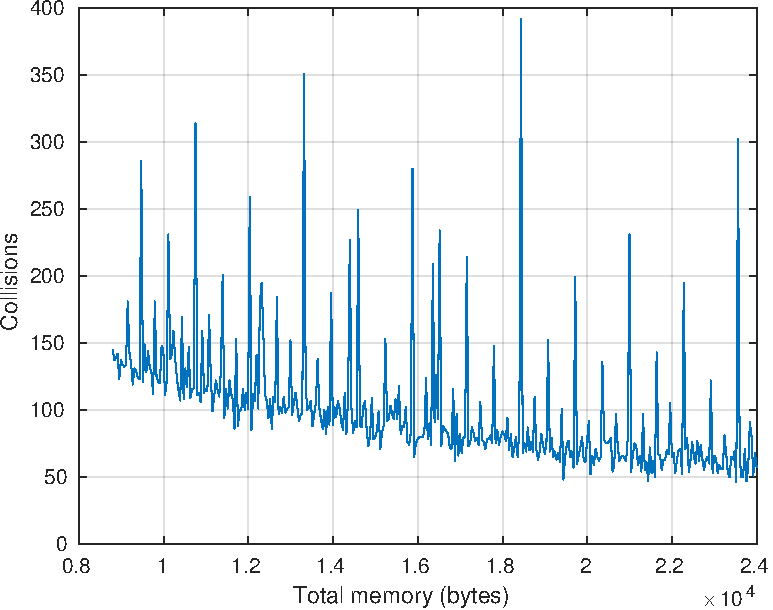
\includegraphics[width=\linewidth]{\hashtablegrowdir/plots/figure1.pdf} 
		\caption{Número de colisões em função da memória total.}
		\label{fig:htg_col_mem_total}
	\end{subfigure}
	\hspace{0.049\textwidth}
	\begin{subfigure}{0.47\textwidth}
		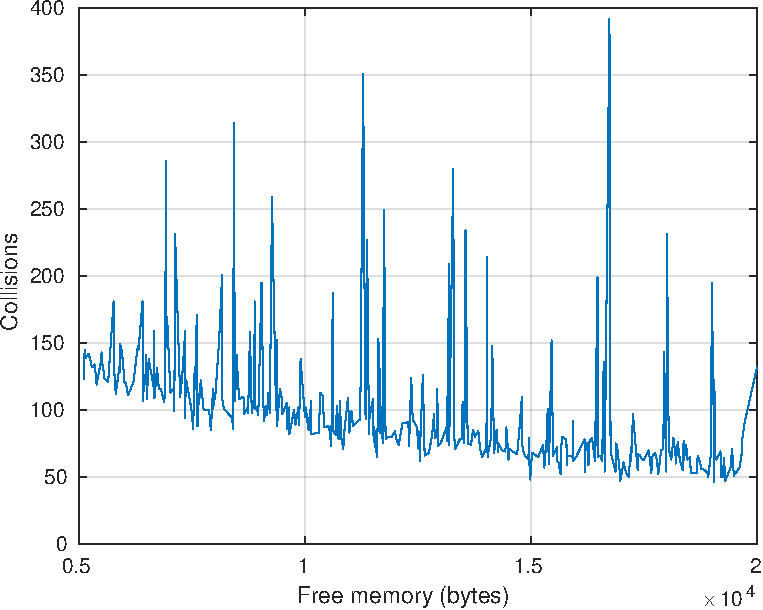
\includegraphics[width=0.96\linewidth]{\hashtablegrowdir/plots/figure2.pdf}
		\caption{Número de colisões em função da memória livre.}
		\label{fig:htg_col_mem_free}
	\end{subfigure}
	
	\caption{Número de colisões em função da memória.}
	\label{fig:htg_col_mem}
\end{figure}

\begin{figure}[h]
	\begin{subfigure}{0.47\textwidth}
		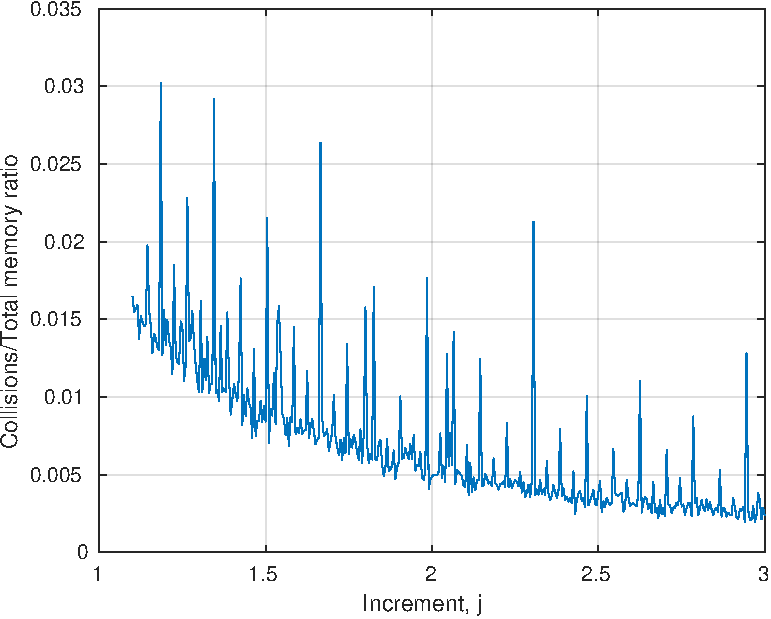
\includegraphics[width=0.96\linewidth]{\hashtablegrowdir/plots/figure3.pdf} 
		\caption{Rácio colisões/memória total.}
		\label{fig:htg_ratio_inc_total}
	\end{subfigure}
	\hspace{0.049\textwidth}
	\begin{subfigure}{0.47\textwidth}
		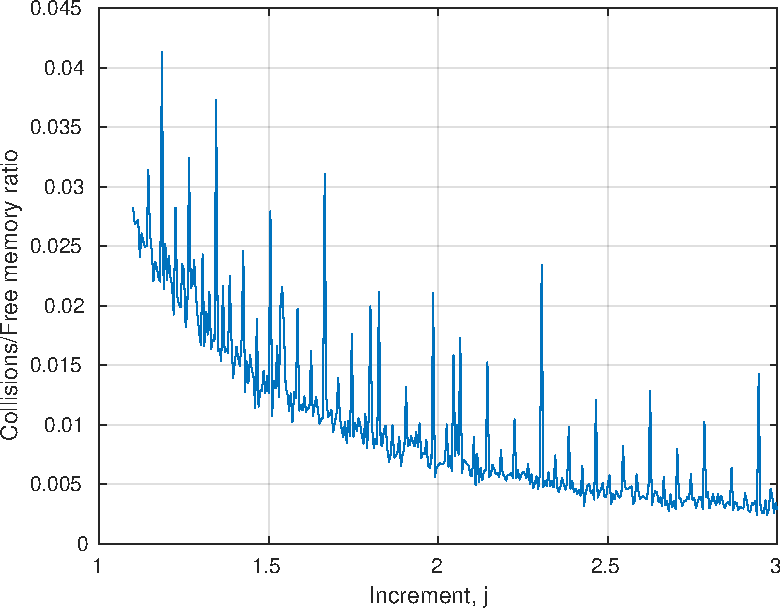
\includegraphics[width=\linewidth]{\hashtablegrowdir/plots/figure4.pdf}
		\caption{Rácio colisões/memória livre.}
		\label{fig:htg_ratio_inc_free}
	\end{subfigure}
	
	\caption{Rácio colisões/memória em função do incremento.}
	\label{fig:htg_ratio_inc}
\end{figure}

\begin{figure}[ht]
	\centering
	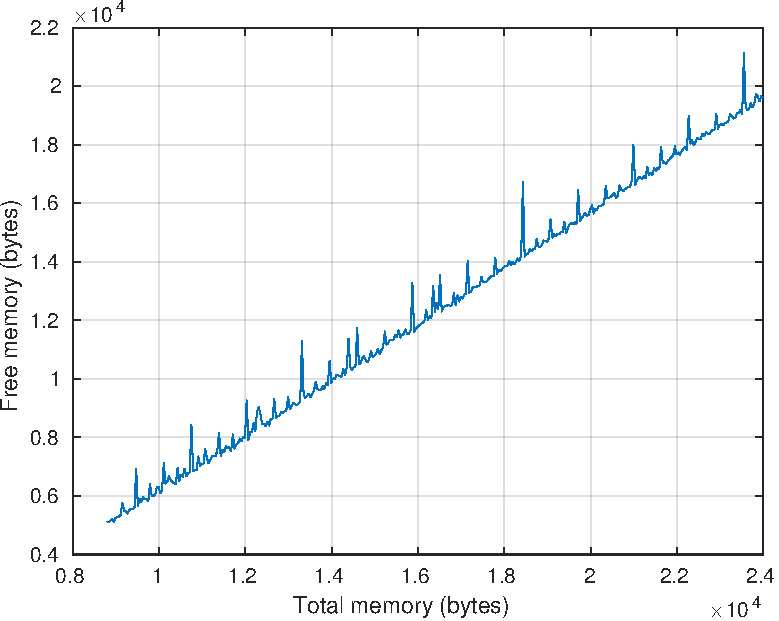
\includegraphics[width=0.47\linewidth]{\hashtablegrowdir/plots/figure5.pdf}
	\caption{Memória livre em função da memória total.}
	\label{fig:htg_free_total}
\end{figure}

\subsection{Análise dos resultados}
Em todos os gráficos, é possível observar irregularidades, associadas a uma maior ou menor quantidade de colisões. Isto deve-se ao facto de a \textit{hash function} não ser perfeita e portanto, consoante o valor de \verb|j|, o índice associado a cada \verb|node| ser diferente.

No entanto, é possível observar que, em geral, o número de colisões diminui com o aumento de memória (ou seja, com incrementos maiores), tal como seria esperado. A relação entre o número de colisões e a memória livre segue a mesma tendência. Em ambos os gráficos, verifica-se uma tendência aproximadamente linear.

Quanto aos rácios colisões/memória em função do incremento, observa-se em ambos os gráficos uma curva descendente, do tipo \begin{math}a \times x^b\end{math}, com \begin{math}-2 < b < -1\end{math}. Por este motivo, verifica-se uma diferença mais acentuada no eixo das ordenadas para incrementos menores do que para incrementos maiores. Assim, considera-se que o melhor incremento é o que apresenta um valor de \begin{math}b\end{math} mais próximo de 2, já que, a partir desse valor, o rácio tende a ser mais constante. Por outro lado, a similariedade entre rácios explica-se pelo facto de a relação entre a memória livre e a memória total ser aproximadamente linear, com um declive próximo de 1 (ver figura \ref{fig:htg_free_total}).

No que concerne à relação entre a memória livre e a memória total (ambas em \textit{bytes}), apesar das irregularidades, é possível efetuar uma regressão linear, onde se obtém a equação \begin{math}y=0.9583x-3357\end{math}.

Assim, uma vez que os gráficos não são completamente conclusivos quanto ao melhor fator de incremento, escolhemos utilizar o valor 2, já que este constitui um equilíbrio entre o número de colisões e a memória utilizada.

\pagebreak
\section{Código}
\subsection{solution\_word\_ladder.c}
\lstinputlisting[firstline=51]{\srcdir/solution\_word\_ladder.c}
\pagebreak
\subsection{Função hash\_table\_grow que testa o melhor incremento}
\lstinputlisting[firstline=4]{\hashtablegrowdir/latex-hash\_table\_grow-test.c}
\pagebreak
\subsection{Script MATLAB que gera os gráficos para análise da hash\_table\_grow} \label{MATLABcode}
\lstinputlisting[style=Matlab-editor, numbers=none, basicstyle=\small\ttfamily, firstline=5]{\hashtablegrowdir/script.m}
\end{document}
